\documentclass{project}
\usepackage[pdfauthor={N. W. Hardy},pdftitle={Software Engineering Group Project, LaTeX Document Example},pdftex]{hyperref}
\usepackage{graphicx}
\graphicspath{ {images/} }
\begin{document}
\title{Software Engineering Group Project}
\subtitle{Project Plan}
\author{Luke Jones}     
\shorttitle{LaTeX}
\version{1.0}
\status{Draft}
\date{2015-10-21}
\configref{SE-12-PM-01}
\maketitle
\tableofcontents
\newpage
\section{INTRODUCTION}
\subsection{Purpose of this Document}
The purpose of this document is to outline our project plan, to provide data on the time frame in which tasks are to completed and to provide information on risks associated with the project, and how their effects may be mitigated.
\subsection{Scope}
This document specifies the time frame in which we aim to begin and complete tasks and the team member(s) who will work on each task. This document also highlights any risks involved with the project with regard to delays, and includes instruction on how the effects of such delays can be mitigated.
\\[1\baselineskip]This document should be read and closely monitored by all project members. It is assumed that the reader is already familiar with QA document SE.QA.05b [1].
\subsection{Objectives}
The objectives of this document are as follows:
\begin {itemize}
	\item To provide group members with a prior knowledge of when major milestones will be targeted.
	\item Illustrate the optimal dates for the beginning and completion of tasks/subtasks.
	\item Outline group member(s) who will be responsible for the completion of each task.
	\item Identify parts of the plan with potential to cause delay, as well as any outside factors that could make task completion longer than necessary.
	\item Advise on course of action in the event of a delay occurring.
\end {itemize}	
\newpage
\section{GANTT CHART}
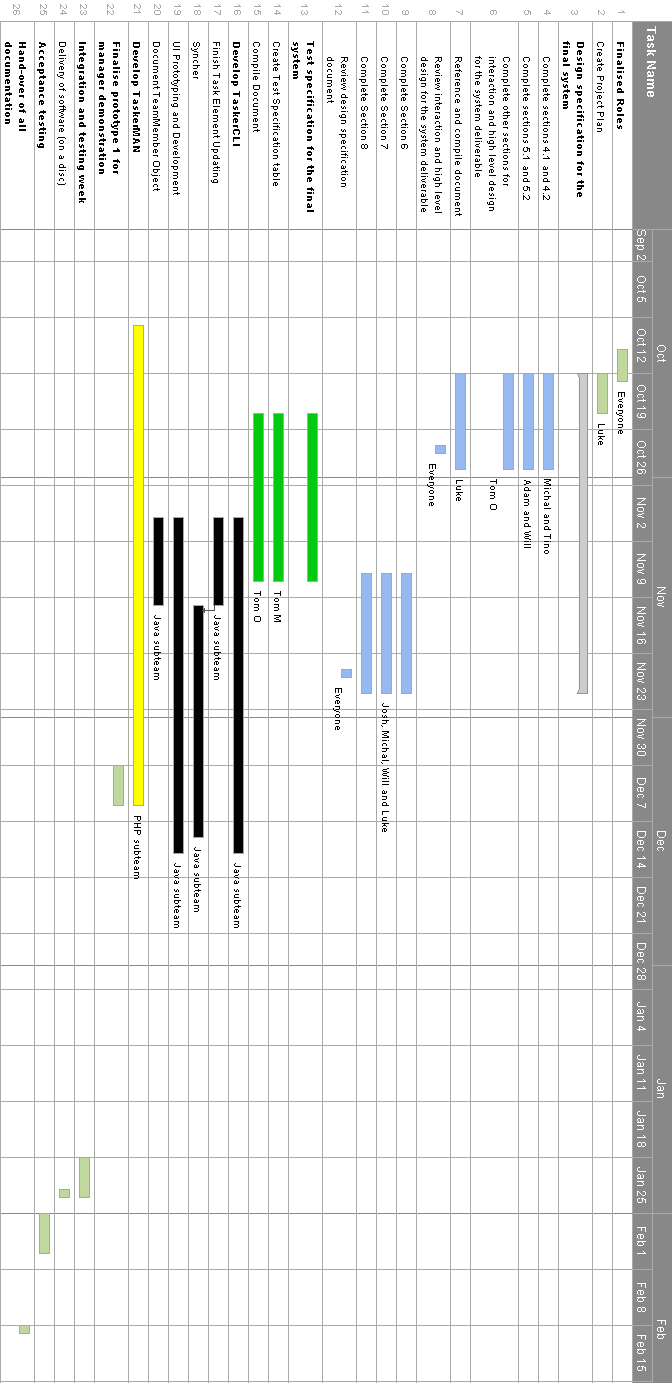
\includegraphics{Ganttchart}
\newpage
\section{RISK ANALYSIS}
\begin{tabular}{ | l || p{8cm} |  }
  \hline
  \textbf{Risk} & \textbf{Instruction on mitigating risk effect} \\ \hline
  Illness to member(s) of group & Agile workload distribution i.e other members can be reallocated other member' roles.\\ \hline
  Members not uploading to GitHub & Disciplinary action overseen by project leader \\ \hline
  Unit testing not adequate & Have a testing team compromised of several members with a wide skill range \\ \hline
  Failure to understand brief requirements & Have project leader seek clarification from superiors. \\ \hline
  University network malfunctioning & Ensure members have a local backup of any files they are currently working on \\ \hline
  Members go over 80 hour limit & Reallocate workload to members with a lower accumulative time value \\ \hline
  Skill levels are not adequate & Assign members roles based on their strengths \\ \hline
  Members mis-understanding what is asked of them & Have meeting minutes shortly uploaded after every meeting in clear detail. \\
  \hline
\end{tabular}  
\addcontentsline{toc}{section}{REFERENCES}
\begin{thebibliography}{5}
\bibitem{se.qa.03} \emph{Software Engineering Group Projects}
General Documentation Standards.
C. J. Price, N. W. Hardy, B.P. Tiddeman SE.QA.03. 1.8 Release.
\end{thebibliography}
\addcontentsline{toc}{section}{DOCUMENT HISTORY}
\section*{DOCUMENT HISTORY}
\begin{tabular}{|l | l | l | l | l |}
\hline
Version & CCF No. & Date & Changes made to Document & Changed by \\
\hline
1.0 & N/A & 2015-10-22 & Initial creation & Luke Jones\\
\hline
\end{tabular}
\label{thelastpage}
\end{document}
\end{verbatim}
\label{fig:footer}
\end{figure}
\clearpage
\addcontentsline{toc}{section}{REFERENCES}
\begin{thebibliography}{5}
\bibitem{se.qa.03} \emph{Software Engineering Group Projects}
Project Plan Specification Standards.
B. P. Tiddeman, N. Hardy, SE.QA.05b. 1.3.
\end{thebibliography}
\addcontentsline{toc}{section}{DOCUMENT HISTORY}
\section*{DOCUMENT HISTORY}
\begin{tabular}{|l | l | l | l | l |}
\hline
Version & CCF No. & Date & Changes made to Document & Changed by \\
\hline
1.0 & N/A & 2015-10-22 & Initial creation & Luke Jones \\
\hline
\end{tabular}
\label{thelastpage}
\end{document}
